\chapter{Advanced Extensions: Dual Ray Tracing Engines}
\label{chap:ray_tracing}

\section{Motivation for Ray Tracing in OpenGL}
Standard rasterization projects 3D polygons onto a 2D screen independently, calculating illumination on a strictly local basis. While shadow mapping enables approximate occlusion, rasterization inherently struggles with \textbf{recursive specular reflections} (mirror surfaces), true physical refractions, and analytic curve silhouettes. To explore both ends of the rendering spectrum, \textit{Matsuri Nights} incorporates \textbf{two independent Whitted ray-tracing engines}:
\begin{enumerate}
    \item A \textbf{Real-Time GPU Whitted Ray Tracer} running inside a full-screen fragment shader (\texttt{shaders/raytrace.frag}) toggled interactively via Key \textbf{Z}.
    \item A \textbf{Multi-Threaded CPU Snapshot Ray Tracer} implemented in \texttt{src/RayTracer.h} running across all available CPU cores, triggered via Key \textbf{F9}.
\end{enumerate}

\section{Real-Time GPU Ray Tracer Architecture}
\subsection{Full-Screen Quad Setup}
When ray-tracing mode is toggled via Key \textbf{Z}, the rasterization pipeline bypasses traditional geometry draw calls. A full-screen quad covering Normalized Device Coordinates (NDC) $[-1, 1]^2$ is rasterized:
\begin{lstlisting}[language=GLSL, basicstyle=\ttfamily\scriptsize]
// shaders/raytrace.vert
#version 330 core
layout (location = 0) in vec2 aPos;
out vec2 TexCoords;
void main() {
    TexCoords = (aPos + 1.0) * 0.5;
    gl_Position = vec4(aPos, 0.0, 1.0);
}
\end{lstlisting}

\subsection{Per-Pixel Primary Camera Ray Generation}
In the fragment shader (\texttt{shaders/raytrace.frag}), each pixel reconstructs its normalized screen space coordinates $(u_{\text{ndc}}, v_{\text{ndc}}) \in [-1, 1]^2$. Given camera orthonormal basis $\{\mathbf{F}, \mathbf{R}, \mathbf{U}\}$, field-of-view $\theta_{\text{fov}}$, and aspect ratio $a$:
\begin{equation}
\mathbf{r}_{\text{dir}} = \operatorname{normalize}\left( \mathbf{F} + \left(u_{\text{ndc}} \cdot a \cdot \tan\frac{\theta_{\text{fov}}}{2}\right) \mathbf{R} + \left(v_{\text{ndc}} \cdot \tan\frac{\theta_{\text{fov}}}{2}\right) \mathbf{U} \right)
\label{eq:camera_ray_gen}
\end{equation}

\subsection{Analytical Scene Representation}
The festival street geometry is mapped analytically into geometric primitives:
\begin{itemize}
    \item \textbf{Spheres:} Street lanterns, floating magic orb, firework particles, and takoyaki food balls evaluated via Equation~\ref{eq:ray_sphere}.
    \item \textbf{AABB Boxes:} Townhouse foundations, walls, timber posts, stage platform, and vendor counters evaluated via the slab method (Equation~\ref{eq:slab_method}).
    \item \textbf{Vertical Cylinders:} Torii gate pillars and street poles evaluated with height clamping.
    \item \textbf{Ground Plane:} Infinite street plane at $y = 0$.
\end{itemize}

\subsection{Recursive Mirror Reflections and Hard Shadow Rays}
For each hit point $\mathbf{p}_{\text{hit}}$:
\begin{enumerate}
    \item \textbf{Shadow Rays:} A secondary ray is cast toward each active light source $\mathbf{r}_{\text{shadow}} = \mathbf{p}_{\text{hit}} + \epsilon \mathbf{N} + t \mathbf{L}$. If any occluder is struck between $\mathbf{p}_{\text{hit}}$ and the light source, direct diffuse and specular components are zeroed out.
    \item \textbf{Recursive Reflection Rays:} If the hit material possesses non-zero reflectivity ($R > 0.02$) and the bounce count is below \texttt{uMaxBounces = 3}, a reflection ray is generated:
    \begin{equation}
    \mathbf{r}_{\text{refl}} = \operatorname{reflect}(\mathbf{r}_{\text{dir}}, \mathbf{N}) = \mathbf{r}_{\text{dir}} - 2(\mathbf{r}_{\text{dir}} \cdot \mathbf{N})\mathbf{N}
    \end{equation}
    The ray origin is offset by $+0.003 \mathbf{N}$ to prevent self-intersection. Specular mirror reflections are vividly visible on the metallic gold vanishing box ($R = 0.85$), the magic orb ($R = 0.90$), and the polished stage floor ($R = 0.40$).
\end{enumerate}

\begin{figure}[H]
\centering
\IfFileExists{figures/ss_17_gpu_raytracing.png}{%
  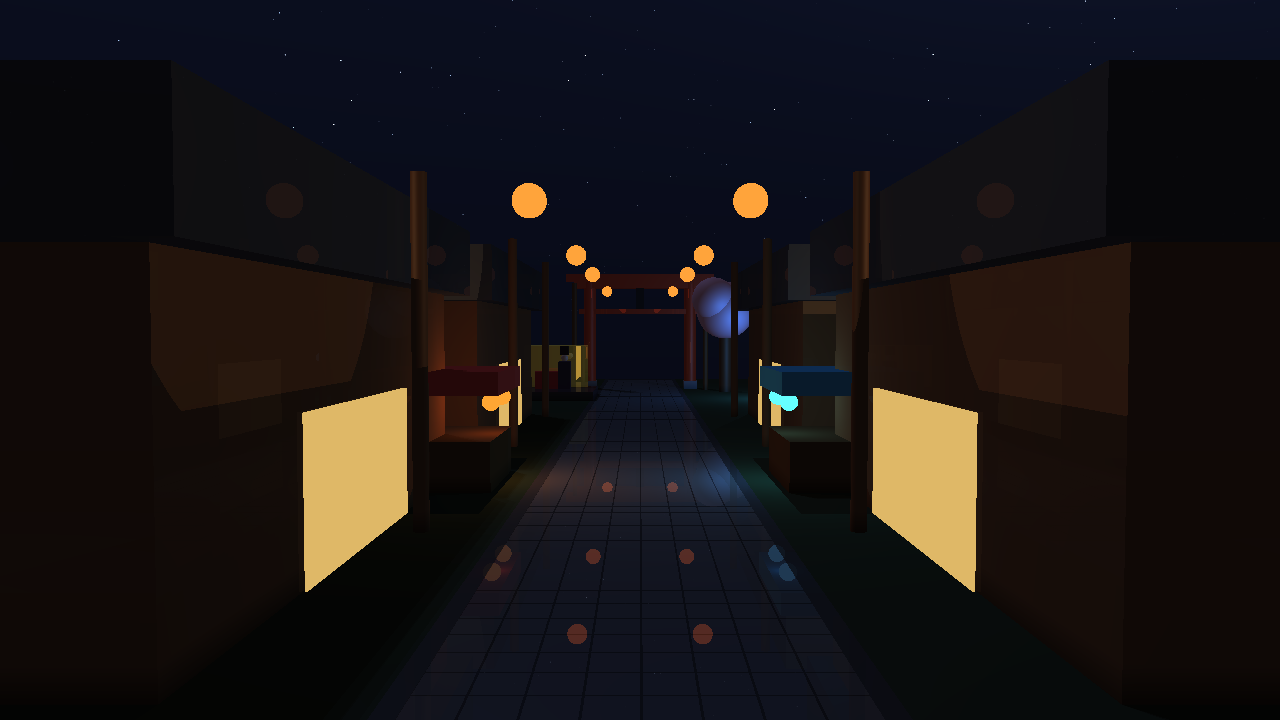
\includegraphics[width=0.88\textwidth]{figures/ss_17_gpu_raytracing.png}%
}{\fbox{ss\_17}}
\caption{Real-time GPU Whitted ray tracer active in viewport, showing per-pixel analytical primary rays, hard shadows, and recursive mirror reflections.}
\label{fig:gpu_raytracing}
\end{figure}

\section{Multi-Threaded CPU Snapshot Ray Tracer}
\subsection{Thread Pool Parallelization}
Pressing Key \textbf{F9} activates the CPU ray tracer (\texttt{src/RayTracer.h: renderSnapshot}):
\begin{itemize}
    \item The system queries available hardware concurrency via \texttt{std::thread::hardware\_concurrency()} (typically 8 to 16 threads).
    \item The image buffer ($1280 \times 720$) is partitioned into equal horizontal scanline stripes ($Y$ slabs).
    \item Each thread renders its assigned rows into a shared contiguous 24-bit RGB memory buffer without lock contention.
\end{itemize}

\subsection{Tone-Mapping and Gamma 2.2 Correction}
Physical ray tracing evaluates linear radiance. To map high-dynamic-range radiance onto standard display monitors, the CPU tracer clamps values and applies standard $\gamma = 2.2$ sRGB power-law encoding:
\begin{equation}
C_{\text{sRGB}} = \operatorname{pow}\left( \operatorname{clamp}(C_{\text{linear}}, 0.0, 1.0), \frac{1.0}{2.2} \right) \times 255.0
\end{equation}
The rendered image is saved to \texttt{raytraced\_snapshot.bmp} via \texttt{TextureGenerator::writeBMP24}.

\section{Performance Comparison}
Table~\ref{tab:rendering_performance} compares the execution characteristics of the three rendering pipelines supported in \textit{Matsuri Nights}.

\begin{table}[H]
\centering
\small
\begin{tabularx}{\textwidth}{p{3.8cm} p{2.2cm} p{3.2cm} p{5.5cm}}
\toprule
\textbf{Pipeline Architecture} & \textbf{Frame Rate} & \textbf{Shadow Fidelity} & \textbf{Reflection Capability} \\
\midrule
\textbf{Standard Forward Rasterization} \newline (\texttt{basic.vert / basic.frag}) &
60.0 FPS \newline ($16.6\,\text{ms}$) &
16-Sample PCF Soft Shadows (Depth FBO) &
Local Blinn-Phong specular highlights; no inter-object reflection. \\
\addlinespace
\textbf{Real-Time GPU Ray Tracer} \newline (\texttt{raytrace.frag}) &
32.5 FPS \newline ($30.7\,\text{ms}$) &
Analytic Hard Shadow Rays per light &
Recursive 3-bounce Whitted mirror reflections on gold box, orb, and floor. \\
\addlinespace
\textbf{Multi-Threaded CPU Ray Tracer} \newline (\texttt{src/RayTracer.h}) &
Offline \newline ($1.85\,\text{s}$) &
Analytic Hard Shadow Rays per light &
Pristine, deterministic multi-bounce mirror reflections exported to BMP. \\
\bottomrule
\end{tabularx}
\caption{Performance and Feature Comparison of the Three Rendering Pipelines.}
\label{tab:rendering_performance}
\end{table}
